\documentclass[10pt,twocolumn]{article}
\usepackage{oxycomps}
\newcommand{\fixme}[2][]{#2}
% overwrite it so it shows up as red
\renewcommand{\fixme}[2][]{\textcolor{red}{#2}}
% overwrite it again so related text shows as footnotes
%\renewcommand{\fixme}[2][]{\textcolor{red}{#2\footnote{#1}}}

% read references.bib for the bibtex data
\bibliography{references}
% include metadata in the generated pdf file
\pdfinfo{
    /Title (Web-Based City Recommender)
    /Author (Anqi Wu)
}

% set the title and author information
\title{Web-Based City Recommender}
\author{Anqi Wu}
\affiliation{Occidental College}
\email{awu2@oxy.edu}

\begin{document}
\maketitle
\begin{abstract}
        
 This project provides an interactive internet site as an assistant for family or individuals who wants to relocate to LA county. By accessing this website, users can discover the cities most suitable for them through filtering attributes (house price, population, number of restaurants, city safeness, climate, and school-related factors) that they might value when making city decisions. In addition, the site presents comprehensible statistics for the users to compare and contrast to filter out the desired results. The construction of the web page involves intended user interviews, web crawling from well-known websites, manipulating data, and user interfaces development.
        
\end{abstract}
\section{Introduction}
 
 As the United States has developed into a global power, it is admitting hundreds of thousands of immigrants worldwide. More specifically, the population of Chinese immigrants in the U.S. has grown to 5.5 per cent of the overall immigrant population. In the past year, China government's policy on Covid-19 and the corresponding strict border control angered the citizens who pursue a liberal democracy, which further strengthened their determination to run away from mainland China. However, most people face the problem of the language barrier and the blocking of information when they are planning to migrate. Therefore, the immigration consultant industry has risen in the past few years, and as the demand increases, the cost of consulting also increases.
\newline
\indent
Since we were the first household to immigrate to the U.S. from our hometown, we received a lot of questions about how we picked the city where we lived. As an earnest person who does not want my friends and family to spend money that is not worthwhile on immigration consultants, I decided to create a free web page that could give them the same assistance a consultant can provide. Combining the consulting process and what I have experienced, I implemented the city-picking procedure into my work with data from more diverse and reliable sources.

\section {Technical Background}

\subsection{Web Crawling}

In reality, not every data set had been organized in a clean spreadsheet like the datasets that kaggle.com provides. Therefore, scientists have to do web data extraction to utilize publicly available web data. In addition, the ability to retrieve data from different websites and compile data has become an essential requirement for data analysts to deal with unstructured data. Web crawling is an automated procedure that scrapes websites to compose a large amount of information since it is much easier to collect a small amount of data by copying and pasting manually instead of spending time constructing a scraping machine. Web scraper is an algorithm built to search the website for the data we are looking for and then extract the requested information from the web page for further analysis. 

\subsubsection{Tools for Web Scraping}
Since this project required web-based data, which needs to translate the type of the data in some cases and is less organized than the numerical data, an automated web scraper is in demand. As a tool that automates web browsing, Selenium is an adequate choice used for web scraping in this project. Although Selenium was initially designed for automated web testing and has a collection of testing appliances, it has a helpful tool called Selenium WebDriver. This webdriver is a system that I can use to create my automated web testing, which I can make use of its automatic characteristic to simulate the web scraping bots.\cite{Mitchell2015Ryan}
\newline
\indent
Although there's a pre-built web crawling robot that can get data from website way faster than web driver using API, Selenium is still the choice for this project. The first reason is that I get the exact value that I am looking for by locating the value from the exact page instead of getting the data from the entire page; the second reason is that sometimes the scraping process requires javascript to click the buttons in order to retrieve the data needed, which API is not capable of doing but Selenium does. Lastly, examining how the webdriver takes control of the laptop and scrolls the webpage by itself and how the data is being scraped down to the spreadsheet is a satisfying and enjoyable experience. 

\subsection{Data Manipulation}
Data manipulation is the process of working on the extracted data or existing dataset and generating another set of data by applying some mathematical operations on it. During the process, Scientists usually first clean up the data by taking away the useless data, or discarding the NaNs (empty values). Then they will rearrange the dataset into the format they want, and restructure the data. Also, they might merge, or separate information based on the demand\cite{Eads2021}. Lastly, they will use their knowledge to perform data analysis on the information, and make the data tell a story that is understandable by the people who are not in the field. 
\newline
\indent
bib

\subsection{Website Scripting}
Website Scripting is constructing pieces of code that will be embedded into the web page, and the script is not visible in the user interface. Furthermore, the scripts will bring a lot of functions like clickable buttons, embedded videos, and other interactive activities. Currently, websites can be split into two categories, which are static and dynamic. A static website will display information exactly the same for different users, which can be constructed using only HTML, and CSS. On the contrary, a dynamic website contains web pages that include information that will change depending on various factors like users' requests, the time zone, product availability...etc. Therefore, different individuals might see different contents from the dynamic webpage based on the users' interactions with the page. The following graph represents the web scripting process visually.
\begin{figure}[h!]
    \centering
    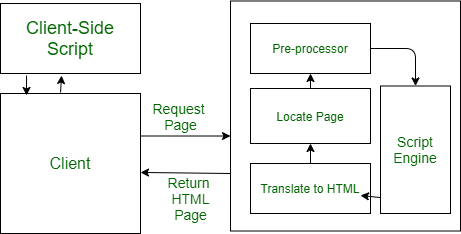
\includegraphics[width=.95\linewidth]{WebScripting.png}
    \small
    \caption{WebScripting Process}   
\end{figure}

\indent
Since this project is designed to help the users to find out the cities that are most suitable for them, which means that the information that will display for each user will be different depending on their decisions, this project is producing a dynamic website using HTML, CSS, and PHP.  

\subsubsection{Hypertext Markup Language}
Hypertext Markup Language is usually abbreviated to HTML, which is the most essential part of the process of building a web worldwide. HTML is the language common to every website and is responsible for taking care of the content layer that will display to users by constructing the structural foundation of the web page\cite{Dean2019}. If someone wants to build his/her own website or web app, he/she has to understand HTML. 
\newline
\indent
Hypertext is any text that can be presented on a computer screen and contains links to other sources or other hypertext documents. A web is a collection of millions of documents, interconnected by hyperlinks. A markup language supplies the interpretation of the text in a document by applying instructions that mark out how text should be laid out, formatted, and structured. In combination, HTML is a markup language the browser operates to reveal information like images, videos, links, and words to the users. Like how people can construct headers, titles, subtitles and hyperlinks in google docs using its formatting options to give the paper an explicit structure, HTML works similarly by giving text formatting instructions to browsers in the configuration of tags called markup. The markup tags are made up of words that are between angle brackets. Changing the words between the angle brackets, it will allow the webpage to display content like graphics, tables, and images. 

\subsubsection{Cascading Style Sheets}
As the second essential element of building a web page, Cascading Style Sheets is responsible for styling by ensuring how elements look on a specific web page, what the color and font of the text are in displaying to the users, and the positioning of the elements. Cascading Style Sheets is usually abbreviated to CSS, and this name comes from how multiple independent style sheets can be operated in a single document simultaneously. For instance, when one style sheet is connecting with one document, it is possible for another style sheet to link to the first style sheet. Therefore, the second style sheet can also be connected to the document the web browser will display. When a collective of style sheets is active and associated with the same document, the browser will run the style in a designated sequence, and the process can be referred to as cascading from one style sheet to the next.
\newline
\indent
 CSS can be categorized into two big categories: Internal Cascading Style Sheets and External Cascading Style Sheets\cite{Fitzgerald2021}. The first one is the style sheet that is located internally in the HTML file that it is associated with. The benefit of using an internal style sheet is that it will improve the performance by minimizing the size of the HTML file, and reducing the bandwidth of the transmission between the CSS file and the HTML file. The external cascading style sheet is the CSS file that are stored separately from the HTML file and can be used in different documents. The advantage of external CSS is that it could help improve web performance by reducing the effort of writing duplicate formatting instructions in different files. CSS can define formatting using rules, and each CSS rule has a selector that tells the HTML file which elements or classes should be selected to apply the CSS properties in the declaration.
\newline
\indent
There are already a lot of well-written UI libraries in the market that website developers can utilize to make their web pages look better. The UI library is used because it speeds up the user interface development process and does not require people to code from scratch. This project uses the UI library called Layui, which has a simple and clean design that I value, and the minimalism concept I believe in.


\subsection{Hypertext Preprocessor and JavaScript}
Hypertext Preprocessor and JavaScript are two widely used web scripting languages for web development. Hypertext Preprocessor, usually known as PHP and originally standing for Personal Home Page, is a website scripting language helpful in developing dynamic websites that Rasmus Lerdorf innovated in 1994\cite{StudySection2019}. The code constructed in PHP is not visible on the webpage since the PHP file is processed before the HTML. By using the PHP language, the content that is displayed to the users will change through multiple forms of user interactions. A PHP script can combine with HTML code or other web frameworks and is executed by the PHP interpreter, which will process the code line by line. After the executing, the web server will send the result to its client. 
JavaScript is another web scripting language that contributes interactive behavior to the web, which is essential for games and applications that require interactive actions. Unlike PHP, JavaScript is capable of working for both the front-end and back-end of the website.
\newline
\indent
Moreover, PHP is more responsible for dealing with problems on the server side. For example, the developer can load the dataset in spreadsheets in various formats to PHP and make them visible to the clients through a library called PHP Excel. The project uses PHP because of its ease of learning, free license, superior delivery for coding and memory usage, and faster page loading speed. On the other hand, JavaScript is more in charge of the problem on the client side of the browser, which the users can see and take action on. For example, associating the external file extension from the JavaScript library jquery.js with the HTML document allows the user to perceive the response when clicking on the interactive buttons or elements, such as the scrolling bar in the table that is displayed on the webpage. 
\newline
\indent
Although JavaScript can be used in both the front and back end of web development, it is more effective to use PHP for the back end because of its shorter learning curve and better security. Nonetheless, since this project does not lean toward either the server or client side, the best strategy is to use both PHP and JavaScript concurrently. 

\section{Prior Work}
There were already numerous websites and applications through the internet that people had built for filtering user demand and comparing the selections they made to find the right product. 

\subsection{The Function of Filtering}
The well-known online directory Yelp is designed for users to discover local businesses. When the user enters the keywords they are looking for, the app will pop out the related companies that match the input. When the users launch the application, they can click on the sorting buttons and set their necessities like the distance from the business to the user's location, the average customer spending, and the business types to search for the results that match their needs. The filtering process in Yelp is also in a prioritized sequence, which means that the second choice that the user makes will be filtering from the results that remain from the previous selection.
\newline
\indent
One of Yelp's popular functions is that it allows users to leave reviews for businesses. However, as more people and businesses are involved in this event, more problems ensue. The company has been put on trial for unfair business practices to increase its revenue\cite{Luca2011}. They are inclined to display more negative reviews under the review sites of businesses that do not buy Yelp's advertising services and conceal the negative reviews from the companies who purchased the advertising services. Also, the review function of this application will lead the companies to hire people to leave positive comments to attract customers. These practices have created a lot of controversies and will become a factor that misguides the users. Under this circumstance, the users will choose the business based on these inaccurate and misleading reviews, which violate the original intention of this application. This project will also include the filtering function but will not implement the function that allows users to comment on the cities to avoid misleading opinions.

	
\subsection{The Feature of Storing Items}
Amazon is another popular client-based website intended to help customers search for the merchandise they are looking for and make purchases. The website will display a list of relevant products by entering the product name or type. After making further selections on the attributes like price range, product brands, and other pertinent factors that the user will concern about, several targeted products will come out, and the users can keep track of the products that interest them by adding them to the cart. However, the users cannot remove the item from the cart on the same page as they added it. When the user accidentally adds a product to the cart, What they need to do to remove it is to go to the cart and click the delete button, which is ineffective and takes a longer time. This project will simulate the adding to cart function, but with a function that can add and remove the item by clicking on the same button on the page. 

\subsection{The Side by Side Data Comparison}
Apple's official website has a page for customers to compare and contrast the different merchandise models. How it works is that the user can select at most three models they want to compare, and the resulting information will be displayed in the other that the Apple website developer had designed. Some of the deficiencies a user may complain about are that they can not compare more models at a time and cannot do further sorting under each data comparison. More specifically, the user cannot compare the models simultaneously if they are interested in ten models; if the user cares more about the display size of the product, they can't sort the size of the product from a larger retina display to a smaller retina display. Thus, this project will avoid these shortcomings by allowing as many items as the user wants to compare at the same time, and also implementing additional sorting buttons on each attribute throughout the filtering process.

\section{Methods}
The goal of this project is to use the collected data on the cities in LA County to help the people who want to pick the right location from those cities by constructing a dynamic website. The first step is to do several rounds of intended user interviews to understand how people decide where they will live. Then, I will know the direction of the data I need and where to get the relevant data. Thus, I can build my scraping robot to obtain the information necessary for my website. After scraping down all the correlated data, the next step is to manipulate it and create algorithms using the data to help the users make decisions. Next, I will start building the user interface that will display my results from data manipulation, have interactive buttons for filtering the information, and other functions that support the city-picking process.

\subsection{User Interview and Interview Results}
This website's intended users will be Chinese who want to start a life in LA County. Therefore, conducting the user interview is necessary for this work. The interview sample came from two sources: the developer's relatives and friends in China and netizens from a Chinese social media platform, Xiaohongshu. 
\newline
\indent
Xiaohongshu is an application that was released in 2019 and is like Instagram in China. As a loyal user of this application since it was released, I am aware of how active the users are on this platform and also how accurate its algorithm is in recommending the posts to the users. Therefore I decided to post a post to collect answers on what factors people will care about when deciding which city to move to. As expected, the post was displayed to the users interested in this topic, and unsurprisingly, a group of enthusiastic netizens commented on my post. Another feature of Xiaohongshu is that it provides the IP address of the users and shows the area where the user is next to their usernames. Thus, I can observe which comments are from the immigrants who have already moved to the U.S. and those who are still in China and want to come. By breaking up the netizens into these two groups, I can focus more on the answers which the IP address in the U.S. because they have more experience and know precisely what people should consider and what they regret not being considered when picking the new city to live in. Moreover, the interview of relatives and friends is through the Chinese instant messaging application WeChat. 
\newline
\indent
After finishing the first round of interviews, I recorded the results from my friend, relatives, and the group of netizens on a spreadsheet with individual names and the factors that will be taken into consideration. I listed all the factors in a row and colored one box green when the factor had once been mentioned. In the end, I counted the number of green boxes under each factor as the number of people who care about the corresponding attribute. By sorting those numbers from high to low, I came to a result indicating that the top 6 factors that will affect people's decision on picking a city are the safeness of the city, the number of Chinese restaurants around,  the quality of education in the area, the house prices, the weather, and the number of people living in the city.
\newline
\indent
The result from the first round of user interviews told me what data I would look for, and after that, I designed the second round of interviews. The goal of the second round of the user interview is to ask the interviewees to elaborate further on the attributes, in other words, the standards that will inspire them to choose from each category. The interview sample in this round is the people who have mentioned one or more of those 6 attributes from the first round of interviews. One of the outcome from the second round of the interview is that the users would like to look at the ranking, student-facaulty ratio, and the student diversity of the school when considering the quality of the education. Using the results from the second round of interviews, I am able to design the sorting metric that will apply to the filtering process on the website. 

\subsection{Obtaining Dataset}
The next essential step of this project is to retrieve the data from reliable sources; I used three methods to gain more experience and insights. 
\newline
\indent
The first method is copying and pasting, which applies to the condition when the data we are looking for has already been organized into a clean table or spreadsheet. Since the result from the second round of interviewing tells that the users are looking for the corresponding crime rate in each city to decide whether a city is safe or not, I started to find resources on the number of crimes in the cities in LA County. Luckily, there's an organized table with the total number of violent crimes, property crimes, and population on laalmanac.com, which will cost me less time to copy and paste the data than to construct a scraping robot for this website. 
\newline
\indent
The second method I used was getting the data by manually counting, which applies to the situation when there's a personal interpretation of the information. In this project, the case would be obtaining the number of Chinese restaurants. My first attempt to get the relevant information is to scrape the Yelp webpage. Still, I realized that there are a lot of well-known Chinese restaurants that exist that are not shown on Yelp. When I clicked on the Chinese food filter tab, many other Asian foods were displayed in the same category. I will get inaccurate data if I scrape this webpage using a scraping robot that can not distinguish between Chinese food and other Asian food. Therefore, I decided to count the Chinese restaurant by hand to avoid this problem and retain the accuracy of the data. I apply this method on google Maps since it is easier to count the red labels on the map than counting through Yelp. I did not perform a scraping robot on google Maps because it has the same problem as Yelp, which will pop out other Asian restaurants when I am looking for Chinese restaurants. Although this hand-counting method of obtaining data is tedious and time-consuming, it is necessary under certain conditions to ensure the accuracy of the data. 
\newline
\indent
The third method I used is constructing web scraping robots using python through Selenium. I perform these robots on redfin.com, USnews.com, and weatherspark.com. Redfin is a real estate website founded in 2004 and has the information that I needed for computing the current average house price that the users will care about. USNews is also a popular website in the U.S. with relevant information on high schools. Weatherspark is a reliable website that offers detailed reports on the weather worldwide, and I can retrieve the average weather of each month in each city as the data for determining the climate of an area. 

\subsubsection{Scraping Robot}
The construction of my scraping robots for the different websites has the same structure, which includes five parts: activating the chrome driver, creating a local workbook, parsing the url, locating the elements, and saving the scraped data into the workbook. Since the data I want might come from the different subpages from the same website, I can obtain the url for the subpages by observing the difference between the urls. For example, the urls for other cities in redfin.com have different suffixes, and each city corresponds to a unique index. By parsing the url and feeding it the unique suffixes for different cities, we will obtain the distinct urls for each city. Then, our robot can control the laptop, open the browser, go to the corresponding page by automatically typing in the url, and then scrape down the information we instructed. 
\newline
\indent
The selenium library provides several strategies to locate the elements that we want to scrape down from a page using the 'find elements' method. The 'find element' method can locate the element by different classes, which is shown in the following graph\cite{geeksforgeeks}. 
\begin{figure}[h!]
    \centering
    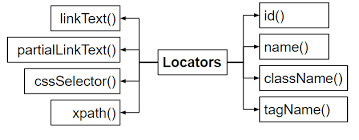
\includegraphics[width=.95\linewidth]{findelement.png}
    \caption{Attributes available for the 'By' class}
    \small
    Selenium provides these methods to locate elements on a page.
\end{figure}
\subsection{Data Processing}
The method I used the most in my scraping code is finding elements by their XPATH, which can be obtained by finding the element in the inspect page and right-clicking to copy its XPath. The XPath of an element refers to its path in the HTML document, which is unique for every element\cite{Viadya2022}. Since the elements I am looking for are in the exact location on the other web pages with information on different cities, I can locate it quickly on other web pages with the same XPath. However, one of the biggest downsides of using XPath is that if the developer modified the website, the XPath of the element will subsequently change, which will be inefficient to go on the inspect page and retrieve the XPath whenever the website has been modified.

The data processing of this project is done by Jupyter Notebook. The first step is to load all the spreadsheets that include the information that I have scraped down into the notebook, and I created a blank excel to store the numerical values needed as the index for the filtering process. After combining the data from different spreadsheets into a single data frame, I started to do some manipulation on each column based on the results from the second round of user interviews. 
\newline
\indent
Since all my interviewees either said that they would prefer a city with more/fewer Chinese restaurants around or prefer a higher ranking when looking at the ranking of the schools, I did not manipulate these two datasets and will sort them in descending and ascending order using the built-in sorting function in PHP.

\subsubsection{Five-Number Summary}
\indent
From the user responses, I realized that when evaluating the city's climate, they would look at the highest and lowest temperature of the city throughout the year, so that they can avoid the city with extremely hot or extremely cold temperatures. The user responses on the climate attribute can also be separated into three categories: cities colder than average, cities with average temperature, and cities warmer than average. To accomplish this implementation, I decided to find the yearly average lowest/highest temperature in each city and set the standard for each category using the 5-number summary. The five-number summary is a helpful method that tells us what the data set looks like by marking the minimum, maximum, median, and value at the first and third quartiles. The first quartile means that there are 25\% of the data points fall below it, and the third quartile means that there are 75\% of the data points fall below it. These two indices are significant in this project because we are comparing the cities, and we would like to know how each city is distributed under each factor. 
\begin{figure}[h!]
    \centering
    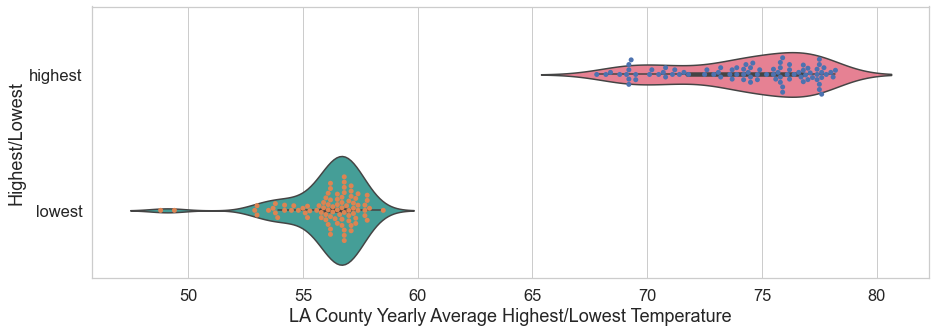
\includegraphics[width=.95\linewidth]{climate.png}
    \caption{Average yearly highest and Average yearly highest temperature}
    \small
    This is a visualization of the 5-number theory on the climate data using the combination of violin plot and swarmplot,
\end{figure}
\indent
Thus, I designed that the cities that have the average temperature to be the cities with yearly average highest temperature(YAH) between the value at the first quartile and the third quartile of the YAH data, and have yearly average lowest(YAL) temperature between the value at the first quartile and the third quartile of the YAL data. The reason behind this is that if we can ensure that the city has both YAH temperature and YAL temperature in the middle fifty of the entire dataset, we can guarantee that those cities won't be extremely hot or cold throughout the year. Following the same logic, the cities that are colder than the average throughout the year should have YAH temperature less than the value at the first quartile of the YAH data and have YAL temperature less than the value at the first quartile of the YAL data; the cities that are warmer than the average throughout the year should have YAH temperature greater than the value at the first quartile of the YAH data and have YAL temperature greater than the value at the first quartile of the YAL data.
\newline
\indent
The other attributes that are also using the 5-number summary to set the standard of filtering are the house price, the population of the cities, and the class size. The feedback from the interviewees indicates that they need information on the average house price, the average population, and the average class size to make a further decision on whether or not they want to pick the specific city. The average house price data is separated into the categories of lower house price, average house price, and higher house price. The population of the city is separated into the categories of small cities, median cities, and large cities. The class size is also separated into the categories of small/medium/large class size by computing the student-faculty ratio. For the above filter categories, I applied the same procedure as how I set the standard for the categories for the weather. 

\subsubsection{Computing the Ratio}
For city safety, my interviewer agreed that they wanted to look at the data on each city's crime rate. Since it is normal for a bigger city to have more crimes, I set the safety standard of whether a city is considered safe or dangerous by taking the ratio between the number of crimes and the population. Therefore, I designed that the safer city would have the ratio of property crime and population and the ratio of violent crime and a population less than the third quartile of both ratios. The dangerous cities will be those with ratios greater than and equal to the third quartile. Therefore, the users who want to settle in a safer city can avoid the city with a relatively higher crime rate. This following graph is a visualization of the number of population vs. the number of of crimes. The black dots represent property crime, and the red dots represent violent crime.
\begin{figure}[h]
    \centering
    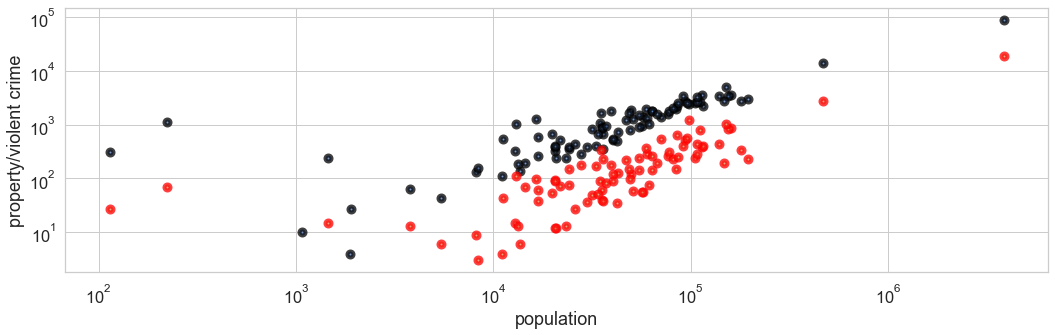
\includegraphics[width=.95\linewidth]{crimerate.png}
    \small
    \caption{Population vs. number of Crimes}
\end{figure}

\subsubsection{Standard Deviation Calculation}
When talking about the diversity of students in the school, the answer from the intended users is either they want to seek education in a less diverse or a more diverse environment. The standard that decides whether a school is diverse is by computing the standard deviation of the races. The schools with a smaller diversity will be the ones with a standard deviation below the medium of the overall race standard deviation, and the schools with a larger diversity will be the ones with a standard deviation above the medium. The graph below is a visual presentation on the percentage of race in each school under the cities with small class size. From the graph, the users can notice how diverse the school is by observing how sparse the dots are.
\begin{figure}[h!]
    \centering
    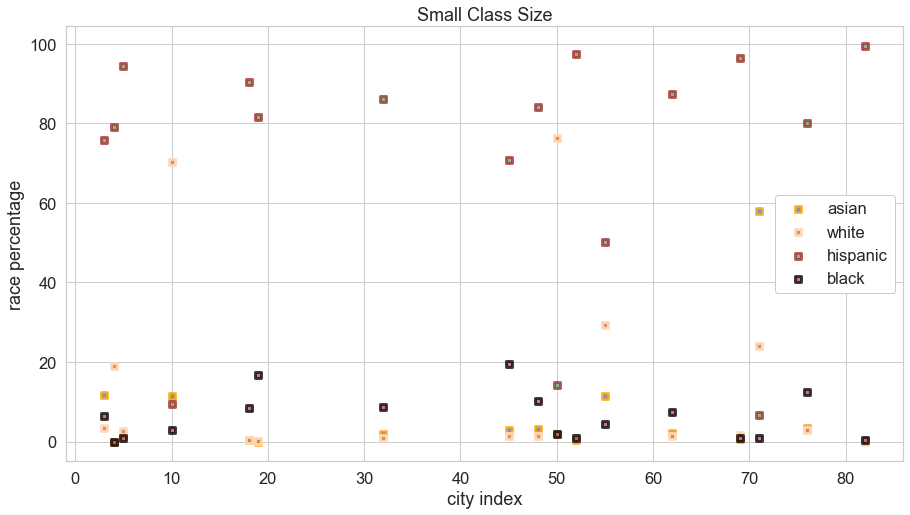
\includegraphics[width=.95\linewidth]{small.png}
    \small
    \caption{School Diversity}
\end{figure}

\subsection{User Interface}
The User interface of this project is composed of a PHPExcel library, a jquery library, a Layui library, a swiper library, three spreadsheets with data, seven PHP files, and eleven HTML files. 
\newline
\indent
The first spreadsheet included the data that will be displayed to the users. The second spreadsheet has the data that was used to compare with the data from the third spreadsheet during the filtering process.

\textbf{Imported Libraries -}
The PHPExcel library is used for loading the data from excel to the website through PHP. The jquery library is used with the swiper library to create the slider bar that will displayed to the user on the website. The Layui library is the pre-built user interface library used to beautify the appearance during the City Picker website development.

\textbf{PHP Files -}
The seven PHP files contain the logic behind each button and include the instructions for loading the data to the website. For example, data.php takes control of loading all the data from the excel files to the website, and the operatType.php is responsible for setting instructions for what information will display to the users when they click on the corresponding sorting buttons. The rest of the PHP files control the characteristic of the different buttons on different pages. For instance, the files set the instructions that when the attribute button has been clicked, it cannot be clicked twice; when clicking the add button to add the city to 'My Cities', the users can click it again to remove it; when the user clicks on the reset button, the PHP file will have the instruction to clear everything.

\textbf{HTML Files -}
Each HTML file represents a page that will display to the users. For example, index.html is the home page of this website and will include a description of the website and some information about LA county. The cityPicker.html is the page where the users will start picking the attributes. The myCities.html is the page where the users can see the cities that they added, and the rest of the eight HTML files correspond to the webpages that will jump to when clicking on the blue attribute buttons. All the HTML are in a similar format: they all start with importing the libraries, setting the style of the elements on the page, displaying the elements, and calling the various functions that will make the elements interactable under the scripting section.

\textbf{Web Hosting -}
In order to have a link for my users to access to the City Picker website, I need to publish my website on the internet through a online service. Web hosting provider will allocate a stable digital repository on the web server for the  websites, and provide a secure space that stores the scripts, images, spreadsheet, and other contents that comprises the website\cite{Pavlovic2020}. I chose to host my website using 000webhost.com because it allow me to publish one website for free by signing up.
\section{Evaluation Metrics}
The evaluation of this work will be based on the website's usability, the data's accuracy, the functionality of the buttons on the website, and the capacity to display the dataset to the users successfully.
\newline
\indent
The usability of the website will evaluate the experience of the users. In other words, how effectively does the website help the users to explore the cities, and do they find the city that best suits their needs? I tested the usability is to send out the link of my website to 10 of my friends who lived in different cities in LA County: San Marino, Agoura Hills, Pomona, Pasadena, Arcadia, San Gabriel, Temple City, Monrovia, Los Angeles and Malibu. Then, I have them perform the process of how they decide to pick the current city they live in. The result showed that eight out of ten people did see their cities on the list at the end of the filtering process, indicating that City Picker's usability is pretty practical. In addition, this approach also shows the pass of the data accuracy test; otherwise, the users won't have the right city that they are looking for on the final list.

The website's functionality and the capacity to display the data set are evaluated by relatives and friends from China. Since they are the intended users, they will probably click on all possible buttons on the page to explore the cities. Therefore, I have them report any issues they encounter when using the websites: such as the buttons not responding and wrong information displaying (i.e. when they are exploring the city's temperature, the number popped out is the data on the house price). I also asked users to recommend other functions that might be helpful for their exploring process.

\subsection{Evaluation Result and Discussion}
The feedback on the website's usability from my friends in the U.S. are overall positive, and the two people who did find their city at the end reported that the final list they got contained the cities they had considered. However, they choose the current city they live in because of their personal preferences, such as the house they live in has a higher price than their original budget. Still, the design of the house is what they like, so they are willing to raise the initial budget for it. From the feedback, my explanation is that City Picker does not guarantee that the cities from the final list are where the users will live since there are a lot of other uncertainties in the world. 
\newline
\indent
The response from the functionality evaluation of the website is valuable, which helped me with the debugging process, and added a new function to the website. One of the testers reported that when he clicked the attribute button, the final list that came out had more cities than the previous list, which cleared out the list of cities that he had been filtered out. This is a careless misconstruct of the instruction code under that specific button, which I fixed immediately after receiving the feedback. Furthermore, the testers also recommended I add a delete button on the 'My Cities' page for each of the cities that had been added so that they can remove the city that they are not satisfied with while exploring the city by clicking on the more buttons. I also agree with them, so I have added that function to the 'My City' page. Lastly, I also got feedback that suggested I refrain from using abbreviations in the table. My response is that if I did not use an acronym, the table would be unimaginably long and inefficient for data comparison. My solution is to add a key to the abbreviation outside of the table with instructions so that the users can check out the complete form while comparing the cities.
\subsubsection{Limitations}
\textbf{Interview Sample Size - }
One of the limitations is the interview sample size. If the interview sample size of this project is more extensive, I will have a lot more feedback and thus will come to a more accurate conclusion. A larger sample size will help me identify outliers more efficiently and provide smaller error margins.
\newline
\textbf{Data Update - } 
The other limitation will be the real-time update of the data. Since the availability of the house and its house price will change over time, I need to update the average house price data more frequently to ensure the accuracy of the data. The outdated data might result in a misleading decision.

\section{Ethical Considerations}
Like all the other sorting engines, City Picker does not guarantee the cities from the final list are the best option for the users to live in because humans are not machines, and their decisions will be affected by other uncertainties that vary among people.

The web scraping process in this project will raise legal and ethical concerns and be regarded as cybercrime if the data scraped are not public data\cite{Day2022}. If the scraping robot is scraping some private data without consent, it will be considered stealing copyright information or hacking the website. Therefore, the data scraped for this project are all from public sources, and scrapers are not designed to attack any websites. Thus, it is free of cyber-security and data privacy.

\section{Future Works}
The City Picker website will be more supportive and accurate when there is a larger sample size. One of the future objectives will be conducting more interviews and enlarging the sample size as much as possible. More feedback from the intended users will directly affect the precision of the sorting process. 
\newline
\indent
Another future goal is to make City Picker more diverse and open to more people from every part of the world. Therefore, more user interviews need to be conducted so that I will know how people who grew up from various backgrounds will make their choices when selecting the city for residence. A resulting function that will be added will let people choose the country they came from, and the website will lead them to the corresponding page with different attributes.
\newline
\indent
Additionally, more cities from different counties or states will be added as future objectives. This will make the website more extensive and provide more options for people to choose from. \newline
\indent
Lastly, building a machine that will obtain data in real time from the resources and load the data to the website automatically in the future will significantly improve the accuracy of the data, which will be valuable for the city-picking process.

\section{Conclusion}
The City Picker website can help users narrow down their choices of cities while clicking on the various filtering options. This web page provides data from reliable sources that the intended users might need help accessing or have trouble finding out where to look for. Furthermore, the data are displayed in an organized table for the users to compare between the cities, making the exploring process more efficient than jumping between different websites to look for the information. Last but not least, City Picker also provides a function for the users to keep track of the cities that interest them so that they will stay aware of the vast choices. Overall, this project works out very well based on the users' feedback and efficiently supports the people who want to relocate to LA County.

\printbibliography

\end{document}